\chapter{Beispiele}
\label{chap:anh_beispiele}


\section{Allgemein}
\label{sec:anh_beispiel_1}
\subsection{Allgemein}
\label{ssec:anh_beispiel_a_1}

\begin{lstlisting}[caption={Abfragen auf Relationswerte},captionpos=b,language=SQL]
?p a owl:Class?
	rdfs:subClassOf pg:Programm?
	rdfs:subClassOf ?restriction.
		?restriction owl:onProperty pg:verwendetProgrammiersprache.
		?restriction owl:hasValue pg:Deklarativ.
?p a owl:Class?
	rdfs:subClassOf pg:Programm?
	rdfs:subClassOf ?restriction.
		?restriction owl:onProperty pg:bestehtAus.
		?restriction owl:someValuesFrom pg:Axiom.
\end{lstlisting}

\subsection{Abfragen auf Relationswerte}
\label{ssec:anh_beispiel_a_2}

\begin{lstlisting}[caption={Alle Programmiersprachen, welche von einem Programm
verwendet werden, welches aus Axiomen besteht},captionpos=b,language=SQL]
PREFIX rdf: <http://www.w3.org/1999/02/22rdfsyntaxns#>
PREFIX owl: <http://www.w3.org/2002/07/owl#>
PREFIX xsd: <http://www.w3.org/2001/XMLSchema#>
PREFIX rdfs: <http://www.w3.org/2000/01/rdfschema#>
PREFIX pg:
<http://www.semanticweb.org/sosterwalder/ontologies/2014/9/programming#>
SELECT *
WHERE {
	?ps pg:wirdVerwendetVon ?o.
	?o pg:bestehtAus pg:axiom.
#pg:Programm ?xx ?object
}
\end{lstlisting}


\subsection{Alle Einsatzgebiete welche in Programmen zum Einsatz kommen,
welche aus Axiome bestehen}
\label{ssec:anh_beispiel_a_3}

\begin{lstlisting}[caption={Alle Einsatzgebiete welche in Programmen zum Einsatz kommen,
welche aus Axiome bestehen},captionpos=b,language=SQL]
PREFIX rdf: <http://www.w3.org/1999/02/22rdfsyntaxns#>
PREFIX owl: <http://www.w3.org/2002/07/owl#>
PREFIX xsd: <http://www.w3.org/2001/XMLSchema#>
PREFIX rdfs: <http://www.w3.org/2000/01/rdfschema#>
PREFIX pg: 
<http://www.semanticweb.org/sosterwalder/ontologies/2014/9/programming#>
SELECT *
	WHERE {
	?es a owl:Class?
		rdfs:subClassOf pg:Einsatzgebiet.
	?r a owl:Restriction?
		owl:onProperty pg:hatEinsatzgebiet?
		owl:allValuesFrom ?es.
	?x a ?es.
	?p a pg:Programm?
		a ?r?
		pg:bestehtAus pg:axiom.
}
\end{lstlisting}

\subsection{Alle Einsatzgebiete welche in deklarativen Programmen zum
Einsatz kommen}
\label{ssec:anh_beispiel_a_4}

\begin{lstlisting}[caption={Alle Einsatzgebiete welche in deklarativen Programmen zum
Einsatz kommen},captionpos=b,language=SQL]
PREFIX rdf: <http://www.w3.org/1999/02/22rdfsyntaxns#>
PREFIX owl: <http://www.w3.org/2002/07/owl#>
PREFIX xsd: <http://www.w3.org/2001/XMLSchema#>
PREFIX rdfs: <http://www.w3.org/2000/01/rdfschema#>
PREFIX pg: 
<http://www.semanticweb.org/sosterwalder/ontologies/2014/9/programming#>
SELECT Distinct ?x
	WHERE {
	?es a owl:Class? rdfs:subClassOf pg:Einsatzgebiet.
	?r a owl:Restriction? 
		owl:onProperty pg:hatEinsatzgebiet? 
		owl:allValuesFrom ?es.
	?x a ?es.
	?p a pg:Programm?
		a ?r.
		#pg:bestehtAus pg:axiom.
	FILTER (regex(str(?p), "deklarativesProgramm","i"))
}
\end{lstlisting}

\section{Wie ist Prolog aufgebaut?}
\label{sec:anh_beispiel_b}

\subsection{Aus was besteht Prolog?}
\label{ssec:anh_beispiel_b_1}
\begin{lstlisting}[caption={Aus was besteht Prolog?},captionpos=b,language=SQL]
PREFIX rdf: <http://www.w3.org/1999/02/22rdfsyntaxns#>
PREFIX owl: <http://www.w3.org/2002/07/owl#>
PREFIX xsd: <http://www.w3.org/2001/XMLSchema#>
PREFIX rdfs: <http://www.w3.org/2000/01/rdfschema#>
PREFIX pl: 
<http://www.semanticweb.org/mira/ontologies/2014/9/untitledontology7#>
SELECT * WHERE {
	?x rdfs:subClassOf pl:Programmiersprache.
	?r a owl:Restriction?
		owl:onProperty pl:hatSyntaxElement?
		owl:someValuesFrom ?t.
	?e rdfs:subClassOf ?t.
}
\end{lstlisting}

\newpage
\subsection{Aus was bestehen logische Elemente?}
\label{ssec:anh_beispiel_b_2}
\begin{lstlisting}[caption={Aus was bestehen logische Elemente?},captionpos=b,language=SQL]
PREFIX rdf: <http://www.w3.org/1999/02/22rdfsyntaxns#>
PREFIX owl: <http://www.w3.org/2002/07/owl#>
PREFIX xsd: <http://www.w3.org/2001/XMLSchema#>
PREFIX rdfs: <http://www.w3.org/2000/01/rdfschema#>
PREFIX pl: 
<http://www.semanticweb.org/mira/ontologies/2014/9/untitledontology7#>
SELECT * WHERE {
	?x rdfs:subClassOf pl:Programmiersprache.
	?r a owl:Restriction?
		owl:onProperty pl:hatSyntaxElement?
		owl:someValuesFrom ?t.
	?e rdfs:subClassOf ?t.
}
\end{lstlisting}

\subsection{Was für sprachliche Elemente verwendet Prolog?}
\label{ssec:anh_beispiel_b_3}
\begin{lstlisting}[caption={Was für sprachliche Elemente verwendet Prolog?},captionpos=b,language=SQL]
PREFIX rdf: <http://www.w3.org/1999/02/22rdfsyntaxns#>
PREFIX owl: <http://www.w3.org/2002/07/owl#>
PREFIX xsd: <http://www.w3.org/2001/XMLSchema#>
PREFIX rdfs: <http://www.w3.org/2000/01/rdfschema#>
PREFIX pl: 
<http://www.semanticweb.org/mira/ontologies/2014/9/untitledontology7#>
SELECT * WHERE {
	?x rdfs:subClassOf pl:Programmiersprache.
	?r a owl:Restriction?
		owl:onProperty pl:hatSyntaxElement?
		owl:someValuesFrom ?t.
	?e rdfs:subClassOf ?t.
	?el rdfs:subClassOf ?e.
	?xa a ?el.
}
\end{lstlisting}


\section{Wie funktioniert Unifkation?}
\label{sec:anh_beispiel_c}

\textit{Erwartete Antwort: In Prolog wird versucht mit Hilfe von Unifikation Anfragen mit Regeln oder Fakten identisch zu machen.}

Da wir von der Fragestellung her wissen, dass wir die Klasse Unifikation wollen, geben wir diese bereits als Filter an.

\subsection{Schritt 1: Beziehungen der Klasse Unifikation nach oben herausfinden}
\label{ssec:anh_beispiel_c_1}

\begin{lstlisting}[caption={Beziehungen der Klasse Unifikation nach oben herausfinden},captionpos=b,language=SQL]
SELECT DISTINCT * WHERE {
	?u a owl:Class.
	?p ?b ?u.
	?t ?a ?p.
	
	FILTER (?u=pl:Unifikation)
}
\end{lstlisting}

\begin{figure}[H]
\centering \rotatebox{0}{\scalebox{0.5}[0.5]{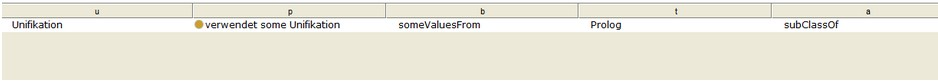
\includegraphics{anhang/bilder/Prolog_1.jpg}}}
\caption{Output: Beziehungen der Klasse Unifikation nach oben herausfinden.\label{fig:prolog_1}\protect\footnotemark}
\end{figure}
\footnotetext{Output Abfrage Protégé}


\subsection{Schritt 2: Beziehungen der Klasse Unifikation nach unten herausfinden}
\label{ssec:anh_beispiel_c_2}

\begin{lstlisting}[caption={Beziehungen der Klasse Unifikation nach unten herausfinden},captionpos=b,language=SQL]
SELECT DISTINCT * WHERE { 
	?u a owl:Class.
	?u rdfs:subClassOf ?y.
	
	FILTER  (?u=pl:Unifikation)
}

\end{lstlisting}

\begin{figure}[H]
\centering \rotatebox{0}{\scalebox{0.5}[0.5]{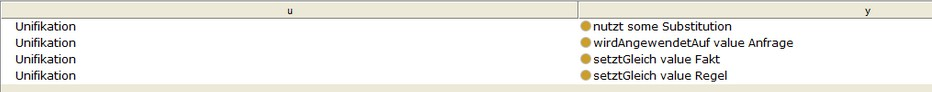
\includegraphics{anhang/bilder/Prolog_2.jpg}}}
\caption{Output: Beziehungen der Klasse Unifikation nach unten herausfinden.\label{fig:prolog_2}\protect\footnotemark}
\end{figure}
\footnotetext{Output Abfrage Protégé}

\subsection{Schritt 3: Details der Beziehungen anzeigen}
\label{ssec:anh_beispiel_c_3}

\begin{lstlisting}[caption={Details der Beziehungen anzeigen},captionpos=b,language=SQL]
SELECT distinct * WHERE { 
	?u a owl:Class.
	?u rdfs:subClassOf ?y.
	?y owl:onProperty ?y3.	
	?y owl:someValuesFrom ?v.
	FILTER  (?u=pl:Unifikation)
}

\end{lstlisting}

\begin{figure}[H]
\centering \rotatebox{0}{\scalebox{0.5}[0.5]{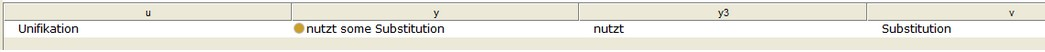
\includegraphics{anhang/bilder/Prolog_3.jpg}}}
\caption{Output: Details der Beziehungen anzeigen.\label{fig:prolog_3}\protect\footnotemark}
\end{figure}
\footnotetext{Output Abfrage Protégé}

\textbf{Feststellung:}\\ Die Beziehungen setztGleich und wirdAngewendetAuf scheinen keine weiteren Relationen zu haben. 


\subsubsection{Zwischenfazit}
\label{sssec:anh_beispiel_c_3_1}

Mit den Schritten 1 bis 3 haben wir festgestellt, dass Unifikation auf Anfragen angewendet wird und diese Fakten und Regeln gleich setzt.\\
Als Verfahren scheint dabei Substitution zum Einsatz zu kommen. Dies muss aber in weiteren Schritten genauer analysiert werden.

\subsection{Schritt 4: Beziehungen der Klasse Substitution herausfinden}
\label{ssec:anh_beispiel_c_4}

\begin{lstlisting}[caption={ Beziehungen der Klasse Substitution herausfinden},captionpos=b,language=SQL]
SELECT distinct * WHERE { 
	?u a owl:Class.
	?u rdfs:subClassOf ?y.
	?y owl:onProperty ?y3.	
	?y owl:someValuesFrom ?v.
	?v rdfs:subClassOf ?v2.
	FILTER  (?u=pl:Unifikation)
}

\end{lstlisting}

\begin{figure}[H]
\centering \rotatebox{0}{\scalebox{0.5}[0.5]{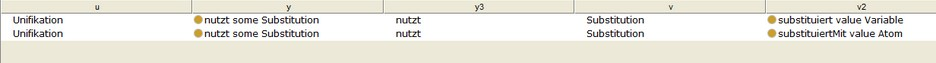
\includegraphics{anhang/bilder/Prolog_4.jpg}}}
\caption{Output: Beziehungen der Klasse Substitution herausfinden.\label{fig:prolog_4}\protect\footnotemark}
\end{figure}
\footnotetext{Output Abfrage Protégé}

\subsection{Schritt 5: Details der Beziehungen anzeigen}
\label{ssec:anh_beispiel_c_5}

\begin{lstlisting}[caption={ Details der Beziehungen anzeigen},captionpos=b,language=SQL]
SELECT distinct * WHERE { 
	?u a owl:Class.
	?u rdfs:subClassOf ?y.
	?y owl:onProperty ?y3.	
	?y owl:someValuesFrom ?v.
	?v rdfs:subClassOf ?v2.
	?v2 owl:onProperty ?y3.	
	FILTER  (?u=pl:Unifikation)
}


\end{lstlisting}

\begin{figure}[H]
\centering \rotatebox{0}{\scalebox{0.5}[0.5]{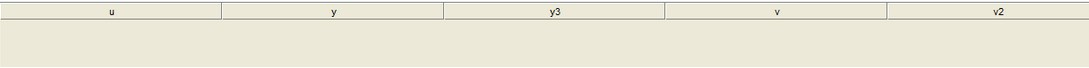
\includegraphics{anhang/bilder/Prolog_5.jpg}}}
\caption{Output: Details der Beziehungen anzeigen.\label{fig:prolog_5}\protect\footnotemark}
\end{figure}
\footnotetext{Output Abfrage Protégé}

\textbf{Feststellung:}\\ Die Beziehungen substituiert und substituiertMit scheinen keine weiteren Relationen zu haben. 

\subsubsection{Zwischenfazit}
\label{sssec:anh_beispiel_c_5_1}

Mit den Schritten 4 und 5 haben wir festgestellt, dass Substitution Variablen mit Atomen substituiert.

\subsection{Schritt 6: Individuen extrahieren}
\label{ssec:anh_beispiel_c_6}

\begin{lstlisting}[caption={Individuen extrahieren},captionpos=b,language=SQL]
SELECT distinct * WHERE { 
	?u a owl:Class.
	?u rdfs:subClassOf ?y.
	?y owl:onProperty ?y3.	
	?y owl:someValuesFrom ?v.
	?v rdfs:subClassOf ?v2.
	?v2 owl:hasValue ?v4.
	
	FILTER  (?u=pl:Unifikation )
}


\end{lstlisting}

\begin{figure}[H]
\centering \rotatebox{0}{\scalebox{0.5}[0.5]{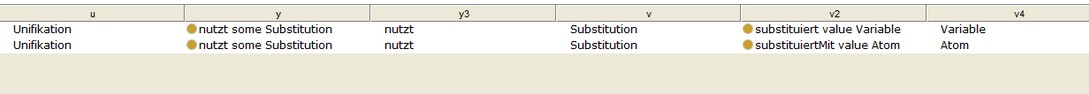
\includegraphics{anhang/bilder/Prolog_6.jpg}}}
\caption{Output: Individuen extrahieren.\label{fig:prolog_6}\protect\footnotemark}
\end{figure}
\footnotetext{Output Abfrage Protégé}

\subsubsection{Fazit}
\label{sssec:anh_beispiel_c_6_1}

Dadurch, dass keine weitere Beziehungen vorhanden sind, haben wir somit alle Beziehungen/Informationen der Unifikation erhalten.

Es stellt sich nun die Frage, wie weitere Informationen zu den Individuen (Variable, Atom, Fakt, Regel und Anfrage) abgerufen werden können.

\section{Was sind Atome?}
\label{sec:anh_beispiel_d}

\textit{Erwartete sparql’sche Antwort: Bei den Atomen handelt es sich um einfache Tokens, wobei diese wiederum Sprachelemente sind. Sprachelemente sind Tokens, woraus Prolog besteht.}

\textit{Erwartete menschliche Antwort: Atome sind Sprachelemente von Prolog, welche mit einem Kleinbuchstaben oder einem Apostrophen beginnen. Atome sind einfache Tokens.
}

Da wir von der Fragestellung her wissen, dass es sich bei Atom um ein sog. owl:NamedIndividual handelt, selektieren wir dieses direkt per Filter.

\subsection{Schritt 1: Atom-Objekt selektieren}
\label{ssec:anh_beispiel_d_1}

\begin{lstlisting}[caption={Atom-Objekt selektieren},captionpos=b,language=SQL]
SELECT distinct * WHERE { 
	?i a owl:NamedIndividual.
	
	FILTER  (regex(str(?i),"atom","i") )
}
\end{lstlisting}

\begin{figure}[H]
\centering \rotatebox{0}{\scalebox{0.5}[0.5]{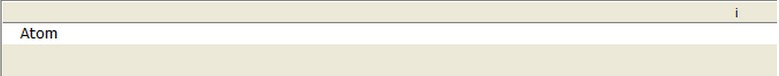
\includegraphics{anhang/bilder/Atom_1.jpg}}}
\caption{Output: Atom-Objekt selektieren.\label{fig:atom_1}\protect\footnotemark}
\end{figure}
\footnotetext{Output Abfrage Protégé}


\newpage
\subsection{Schritt 2: Klasse/Typ des Individuums herausfinden}
\label{ssec:anh_beispiel_f_2}

\begin{lstlisting}[caption={Klasse/Typ des Individuums herausfinden},captionpos=b,language=SQL]
SELECT distinct * WHERE { 
	?i a owl:NamedIndividual.
	?i a ?c.
	
	FILTER  (regex(str(?i),"atom","i") )
}
\end{lstlisting}

\begin{figure}[H]
\centering \rotatebox{0}{\scalebox{0.5}[0.5]{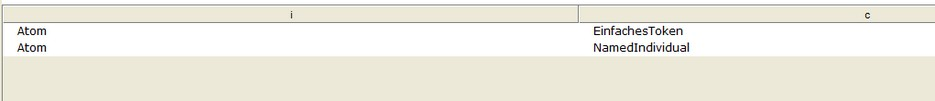
\includegraphics{anhang/bilder/Atom_2.jpg}}}
\caption{Output: Klasse/Typ des Individuums herausfinden.\label{fig:atom_2}\protect\footnotemark}
\end{figure}
\footnotetext{Output Abfrage Protégé}

\textbf{Feststellung:}\\  Bei den Atomen handelt es sich um einfache Tokens (und um eine NamedIndividual, was aber bereits im Vorfeld klar war).

\subsection{Schritt 3: Beziehungen des einfachen Token herausfinden}
\label{ssec:anh_beispiel_f_2}

\begin{lstlisting}[caption={Beziehungen des einfachen Token herausfinden},captionpos=b,language=SQL]
SELECT distinct * WHERE { 
	?i a owl:NamedIndividual.
	?i a ?c.
	?c ?xx ?z. 	# Gibt alle Beziehungen aus
	
	FILTER  (regex(str(?i),"atom","i") && ?c=pl:EinfachesToken)
}
\end{lstlisting}

\begin{figure}[H]
\centering \rotatebox{0}{\scalebox{0.5}[0.5]{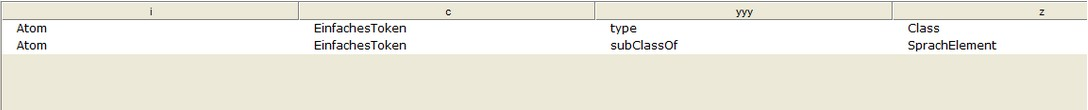
\includegraphics{anhang/bilder/Atom_3.jpg}}}
\caption{Output: Beziehungen des einfachen Token herausfinden.\label{fig:atom_3}\protect\footnotemark}
\end{figure}
\footnotetext{Output Abfrage Protégé}

\textbf{Feststellung:}\\ Wir sehen, dass einfache Tokens die Prädikate type und subClassOf mit den Subjekten Class bzw. SprachElement hat. Dies erlaubt nun die Einschränkung des Queries auf den Teil von Interesse, also subClassOf.

\begin{lstlisting}[caption={Beziehungen des einfachen Token herausfinden 2},captionpos=b,language=SQL]
SELECT distinct * WHERE { 
	?i a owl:NamedIndividual.
	?i a ?c.
	?c rdfs:subClassOf ?z.
	
	FILTER  (regex(str(?i),"atom","i") && ?c=pl:EinfachesToken)
}

\end{lstlisting}

\begin{figure}[H]
\centering \rotatebox{0}{\scalebox{0.5}[0.5]{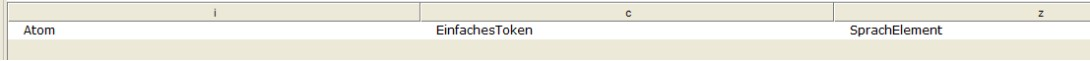
\includegraphics{anhang/bilder/Atom_3_b.jpg}}}
\caption{Output: Beziehungen des einfachen Token herausfinden 2.\label{fig:atom_3_b}\protect\footnotemark}
\end{figure}
\footnotetext{Output Abfrage Protégé}

\textbf{Feststellung:}\\  Einfache Tokens scheinen also Sprachelemente zu sein.

\subsection{Schritt 4: Beziehungen der Klasse SprachElement herausfinden}
\label{ssec:anh_beispiel_f_4}

\begin{lstlisting}[caption={Beziehungen der Klasse SprachElement herausfinden},captionpos=b,language=SQL]
SELECT distinct * WHERE { 
	?i a owl:NamedIndividual.
	?i a ?c.

	?c rdfs:subClassOf ?z.
	?z rdfs:subClassOf ?e.
	
	FILTER  (regex(str(?i),"atom","i") && ?c=pl:EinfachesToken)
}
\end{lstlisting}

\begin{figure}[H]
\centering \rotatebox{0}{\scalebox{0.5}[0.5]{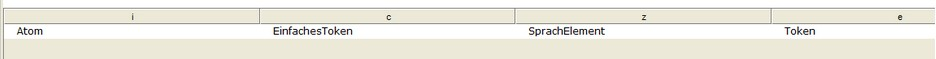
\includegraphics{anhang/bilder/Atom_4.jpg}}}
\caption{Output: Beziehungen der Klasse SprachElement herausfinden.\label{fig:atom_4}\protect\footnotemark}
\end{figure}
\footnotetext{Output Abfrage Protégé}

\subsection{Schritt 5: Beziehungen zu Token}
\label{ssec:anh_beispiel_f_5}

Nachdem wir festgestellt haben, dass Token selbst keine weiteren Relationen mehr hat, wird in diesem Schritt die Anfrage umgedreht.


\begin{lstlisting}[caption={Beziehungen zu Token},captionpos=b,language=SQL]
SELECT distinct * WHERE { 
	?i a owl:NamedIndividual.
	?i a ?c.

	?c rdfs:subClassOf ?z.
	?z rdfs:subClassOf ?e.
	?o ?w ?e.


	FILTER  (regex(str(?i),"atom","i") && ?c=pl:EinfachesToken)
}
\end{lstlisting}

\begin{figure}[H]
\centering \rotatebox{0}{\scalebox{0.5}[0.5]{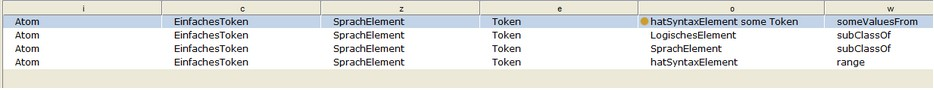
\includegraphics{anhang/bilder/Atom_5.jpg}}}
\caption{Output: Beziehungen zu Token.\label{fig:atom_5}\protect\footnotemark}
\end{figure}
\footnotetext{Output Abfrage Protégé}

\textbf{Feststellung:}\\  Token wird von einer Klasse/einem Objekt mittels der Beziehung hatSyntaxElement als range verwendet.



\subsection{Schritt 6: Objekt(e) mit Relation hatSyntaxElement herausfinden}
\label{ssec:anh_beispiel_f_6}

Es soll herausgefunden werden, welche Objekte das Prädikat hatSyntaxElement als Eigenschaft und Token als Wert einer Einschränkung verwenden.


\begin{lstlisting}[caption={Objekt(e) mit Relation hatSyntaxElement herausfinden},captionpos=b,language=SQL]
SELECT distinct * WHERE { 
	?i a owl:NamedIndividual.
	?i a ?c.
	?c rdfs:subClassOf ?z.
	?z rdfs:subClassOf ?e.
	?bez rdfs:range ?e.
	?r a owl:Restriction;
		owl:onProperty ?bez;
		owl:someValuesFrom ?e.
	?cl rdfs:subClassOf ?r.

	FILTER  (regex(str(?i),"atom","i") && ?c=pl:EinfachesToken)
}
\end{lstlisting}

\begin{figure}[H]
\centering \rotatebox{0}{\scalebox{0.5}[0.5]{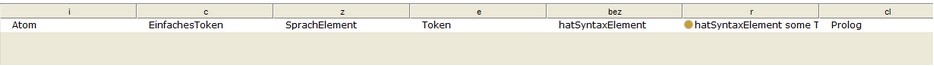
\includegraphics{anhang/bilder/Atom_6.jpg}}}
\caption{Output: Objekt(e) mit Relation hatSyntaxElement herausfinden.\label{fig:atom_6}\protect\footnotemark}
\end{figure}
\footnotetext{Output Abfrage Protégé}

\textbf{Feststellung:}\\  Es handelt sich bei dem gefunden Objekt um Prolog!

\subsection{Schritt 7: Beziehungen zu Prolog herausfinden}
\label{ssec:anh_beispiel_f_7}

Es soll herausgefunden werden, welche Objekte das Prädikat hatSyntaxElement als Eigenschaft und Token als Wert einer Einschränkung verwenden.


\begin{lstlisting}[caption={Beziehungen zu Prolog herausfinden},captionpos=b,language=SQL]
SELECT distinct * WHERE { 
	?i a owl:NamedIndividual.
	?i a ?c.
	?c rdfs:subClassOf ?z.
	?z rdfs:subClassOf ?e.
	?bez rdfs:range ?e.
	?r a owl:Restriction;
		owl:onProperty ?bez;
		owl:someValuesFrom ?e.
	?cl rdfs:subClassOf ?r.
	?cl rdfs:subClassOf ?ccl.
	FILTER  (regex(str(?i),"atom","i") && ?c=pl:EinfachesToken)
}
\end{lstlisting}

\begin{figure}[H]
\centering \rotatebox{0}{\scalebox{0.5}[0.5]{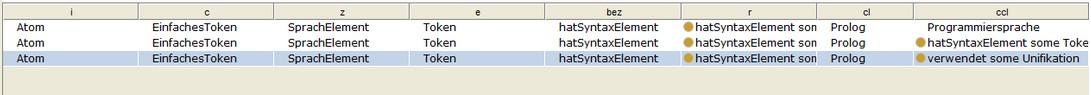
\includegraphics{anhang/bilder/Atom_7.jpg}}}
\caption{Output: Beziehungen zu Prolog herausfinden.\label{fig:atom_7}\protect\footnotemark}
\end{figure}
\footnotetext{Output Abfrage Protégé}

\textbf{Feststellung:}\\  Prolog hat als übergeordnetes Objekt die Klasse Programmiersprache, ist als Unterklasse von dieser. Weiter ist ersichtlich, dass Prolog aus Token Elementen besteht und Unifikation verwendet.

\subsubsection{Zwischenfazit}
\label{sssec:anh_beispiel_c_7_1}

Die gewonnen Erkenntnisse decken die Fragestellung grösstenteils ab, was aber nicht ersichtlich ist, ist, dass Atome über einen kleinen Anfangsbuchstaben verfügen.

\subsection{Schritt 8: Kommentar(e) der Individuen ausgeben}
\label{ssec:anh_beispiel_f_8}

Als Idee zur Lösung zum Zwischenfazit wird die Annotation comment von allen NamedIndividual Objekten ausgegeben.


\begin{lstlisting}[caption={Kommentar(e) der Individuen ausgeben},captionpos=b,language=SQL]
SELECT distinct * WHERE { 
	?i a owl:NamedIndividual.
	?i rdfs:comment ?x.
	FILTER  (regex(str(?i),"atom","i"))
}
\end{lstlisting}

\begin{figure}[H]
\centering \rotatebox{0}{\scalebox{0.5}[0.5]{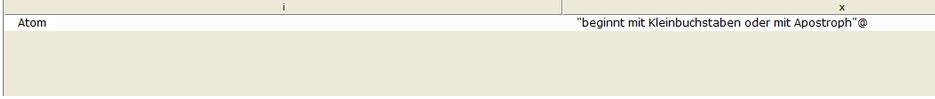
\includegraphics{anhang/bilder/Atom_8.jpg}}}
\caption{Output: Kommentar(e) der Individuen ausgeben.\label{fig:atom_8}\protect\footnotemark}
\end{figure}
\footnotetext{Output Abfrage Protégé}

Analog kann dies natürlich in der Abfrage von Schritt 7 verwendet werden..

\subsubsection{Fazit}
\label{sssec:anh_beispiel_c_8_1}

Die ursprüngliche Frage konnte also erfolgreich wie folgt beantwortet werden:

\begin{itemize}
		\item Atome sind Sprachelemente \\
		Schritt 4
		\item von Prolog\\
		Schritt 6
		\item welche mit einem Kleinbuchstaben oder einem Apostrophen beginnen.\\
		Schritt 8
		\item Atome sind einfache Tokens.\\
		Schritt 3
\end{itemize}

\section{Familienbeispiel}
\label{sec:anh_beispiel_g}

Damit wir eine Bestätigung bekommen, dass unser Semantisches System die gleiche Mächtigkeit wie Prolog (also alle notwendigen Funktionalitäten) besitzt, haben wir ein FamilienProlog Beispiel abgebildet.

Die Situation aus family.pl (siehe \ref{ssec:anh_beispiel_g_prolog}) soll abgebildet werden.


Fakten werden mit Klassen resp. Objekt oder Data Properties abgebildet. Die Argumente in Prolog werden als Individuen abgebildet. (siehe \ref{ssec:anh_beispiel_g_owl}).
Die Regel können eins zu eins übernommen werden.

Die Beispielanfragen wurden genau gleich wie in Prolog beantwortet. 

\begin{lstlisting}[caption={Familienbeispiel in Prolog},captionpos=b,language=SQL]
ASK WHERE {
  	:hans :isAncestor :tea.
 }
\end{lstlisting}

\subsection{Alle Nachfahren von Doris}
\label{ssec:anh_beispiel_g_1}
\begin{lstlisting}[caption={Alle Nachfahren von Doris},captionpos=b,language=SQL]
SELECT
	*
WHERE {
	?subject :isAncestor ?object.
  	#FILTER regex(?subject, "doris", "i")
}
\end{lstlisting}

\subsection{Ist hans vorfahre von tea?}
\label{ssec:anh_beispiel_g_2}
\begin{lstlisting}[caption={Ist hans vorfahre von tea?},captionpos=b,language=SQL]
ASK WHERE {
  	:hans :isAncestor :tea.
 }
\end{lstlisting}

Zusätzlich zu der Möglichkeit anfragen zu stellen zeigt der Reasoner in Protégé seine Folgerungen direkt bei den Objekten an. Der Reasoner konnte in diesem Beispiel dank unserer Regeln direkt erkennen das doris eine Mutter ist und Verfahre von lisa, hans, luca, tea.

\begin{figure}[H]
\centering \rotatebox{0}{\scalebox{0.5}[0.5]{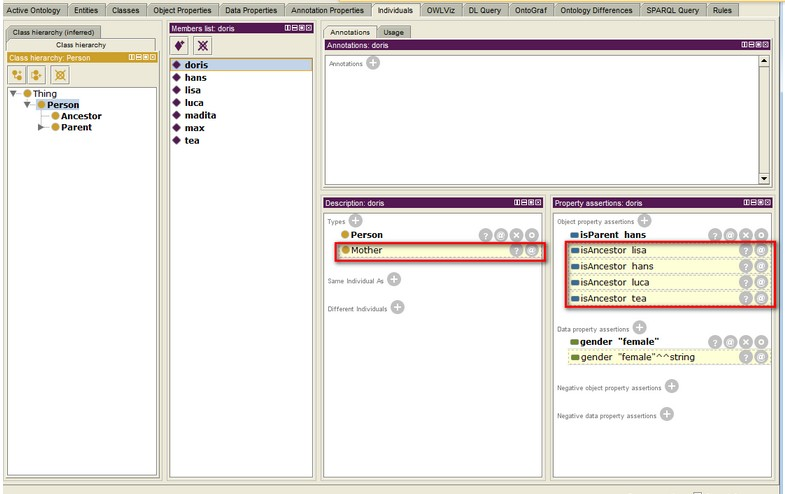
\includegraphics{anhang/bilder/Family.jpg}}}
\caption{Output: Familienbeispiel Anzeige.\label{fig:family}\protect\footnotemark}
\end{figure}
\footnotetext{Reasoning in Protégé}


\subsection{Familienbeispiel in Prolog}
\label{ssec:anh_beispiel_g_prolog}
\lstinputlisting{anhang/family.pl}

\subsection{Familienbeispiel in OWL}
\label{ssec:anh_beispiel_g_owl}
\lstinputlisting[breaklines=true]{anhang/family.owl}



